\section{AWS Elastic Load Balancing [ Author: Aqib Feroz ]}

Load Balancers are basically servers that will front our application and forward all the internet traffic to our instances of our application downstream. 
\begin{figure}[h]
    \centering
    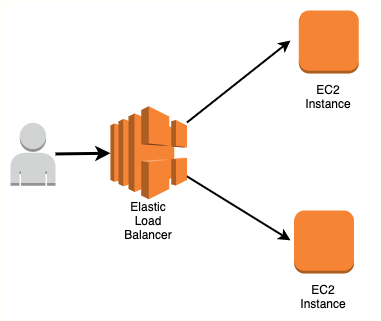
\includegraphics[scale=1.3, width=16cm, height=9cm]{images/load-balancer.png}
    \caption{Load Balancer}
    \label{fig:my_label}
\end{figure}

We have our EC2 instances where we have our application and we have a load balancer a bit before that. When the user connect, it will not connect to the EC2 instances rather the user will connect to the Load Balancer. Similarly we can have multiple users which are connected through elastic load balancers to the EC2 instances.

\textbf{Usage of a Load Balancer [ Author: Aqib Feroz ]}

They spread load across multiple downstream instances so we can scale our instances downstream but expose only a single point of access (DNS) to our application. In a similar way, if one of our downstream instances fails, we do not want our clients and users to see that failure, we want the load balancer to continue to work. So, the load balancer do health checks to our instances to verify that they are working fine and if they do not work fine, it will redirect the traffic to the instances which are working. Health checks are crucial for load balancers, they enable the load balancer to know if instances it forwards traffic to are available to reply to requests, the health check is done on a port and a route, if the response is not 200 (OK), then the instance is unhealthy. Also the Elastic Load Balancer can provide SSL Termination or HTTPS that means the termination and the encryption of the connection between the clients and the Elastic Load Balancer (ELB) and then the ELB goes and talks directly to the instances in HTTP traffic. It can also enforce stickiness with cookies so that means the user basically will talk to the same instances overtime ans there is also a concept of high availability of zones that means the load balances can run across many zones and so do our instances, that basically allows our application to be available in case if an availability zone fails. Load Balancer can also separate public traffic from private traffic. We will discuss further the types Elastic Load Balancer.

\textbf{Application Load Balancer [ Author: Aqib Feroz ]}

Application Load Balnacer are called layers 7 because they operate at the HTTP level, they allow you to handle multiple HTTP applications across machines and we can group these applications in target groups. We can also load balance multiple applications on the same machine in the containers. Load balancing can be done on route in URL or on hostname in URL so we have greater flexibility in choosing the options. Load balancers are great fit for microservices and container based application for example Docker and ECS and also for Amazon EC2 ofcourse. There is also a port mapping feature in which the load balancer can redirect to any dynamic port in the backend and this allows the load balancer to redirect to the same instance on application running on the same machine. In comparison, if we wanted to run five micro services using a classic load balancer, we had to set up five classic load balancer which comes to very expensive and inefficient, but now we have only one load balancer which can front ten applications.
With ALB, we can enable stickiness at the target group level so that means the same user request goes to the same instance and this stickiness is generated by ALB so it will add a cookie at the ALB level. Application Load Balancer supports HTTP, HTTPS and websockets protocols.

\textbf{Network Load Balancer [ Author: Aqib Feroz ]}

Network Load Balancers are layer 4 Load balancers which are the network layer of the system and they handle TCP traffic with the help of target groups. So, we can create multiple target groups based upon the port which we want to communicate. Network Load Balancer also works at VPC level and can be routed on multiple ports. NLB cannot support Lambda function and we have to create a static IP per subnet, there will be an option given while creating the network load balancer we have to create a static IP for network layer. These are low latency and high throughput Load balancers, we can preserve the source IP address for non-http apps. NLB do not support HTTP/2.

\textbf{Gateway Load Balancer [ Author: Aqib Feroz ]}

Gateway Load Balancer is the newest addition to the Elastic Load Balancer portfolio. GWLB handles all the  IP traffic packet by packet and used with third party appliances. It's a gateway and a load balancer, we can say it is the combination of two entities. It provides significant number of opportunities, it opens up a new frontier to deploy appliances. When the gateway load balancer receives traffic, then it acts as a layer four load balancer. Gateway Load Balancer (GWLB) get cloud-native elastic scale and availability, without having to solve these complex problems we can focus on the core skill set. We can innovate faster by focusing on core expertise leaving behind solving the problems of cloud-native elastic scale availability service delivery, we can offload this problem to Amazon web services. To summarize, the GWLB is essentially a combination of layer three gateway and a layer four load balancer. The GWLB endpoint is essentially a VPC endpoint that can be a next-hop in route table. We can send out traffic to GWLB using simple route table updates, if we know how to do routing and if we know how to update route tables, then using GWLB is the easy task for us to do.

GWLB provides horizontal scale and fault tolerance to the appliances, we can insert our services transparently because of the layer three encapsulation capabilities. We can share our appliance fleet across VPCs and across accounts.


All the load balancers has instance health check feature so we can check the health check for our registered instances. We can use CloudWatch in all the load balancers which is a built in feature. We can have logging to S3 bucket for all the ELBs. SSL termination support and zonal failover is also a common feature in all Elastic Load Balancers. With IAM policies, we can restrict the permissions as well. 
